\documentclass[runningheads]{llncs}
%
\usepackage{graphicx}
% Used for displaying a sample figure. If possible, figure files should
% be included in EPS format.
%
% If you use the hyperref package, please uncomment the following line
% to display URLs in blue roman font according to Springer's eBook style:
% \renewcommand\UrlFont{\color{blue}\rmfamily}

\begin{document}
%
\title{Distributed Inventory Manager}

\author{Group 14: Johannes Hartmann \and Luca Schwarz \and Marko Juric}

\institute{}
%
\maketitle              % typeset the header of the contribution

\section{Introduction}

As part of the course project an inventory system shall be developed. The system will be a client server architecture where the servers are responsible to keep the data and process updates regarding goods and stock information. The clients can request the currently available goods and the amount and send update information if new goods are available or if goods are taken out of stock. For the updates it’s important to ensure strong consistency and ordering of events such that all clients have the current information. Within the servers it shall be possible to add additional nodes to the system dynamically and to handle different failure cases while still being able to process requests.


\section{Project Requirements Analysis}

\subsection{Architectural Description}

Client-Server Architecture: Our system will adopt a client-server model, which consists of multiple clients interfacing with a cluster of server nodes. The clients are responsible for querying current stock levels and submitting updates for processing. The server nodes serve these stock level requests and manage inventory updates. Amongst the server nodes, a leader will be elected to coordinate updates and ensure consistency across the distributed system.

\subsection{Dynamic Discovery of Hosts}
Server-side: Upon initiation, each server node will broadcast its presence and listen for existing members of the system to construct a current view of the cluster. This dynamic discovery protocol allows the system to scale horizontally without manual configuration.

Client-side: Clients are designed to automatically detect server nodes in the system. This enables seamless interaction with the inventory system, ensuring that clients can always locate a server node to process their requests.


\subsection{Fault Tolerance}

Our system is engineered to handle different types of failures, ensuring continuous operation:
Leader Failure: If the current leader server fails, the remaining servers will initiate a leader election to select a new leader. This ensures that the system continues to process updates without significant downtime.

Server Crash: In the event of a server crash, client requests are automatically redirected to other operational server nodes. A health check mechanism and a server list update protocol ensure that clients and servers are aware of the available nodes in real-time.

Retry Logic: To handle transient failures, the system will implement a retry mechanism. This ensures that, for instance, during a purchase processing, if a write operation fails, the system will retry the operation. We will have a limit to  prevent excessive retries that could overwhelm the system, allowing it to fail and recover.

\subsection{Voting / Leader Election}

Consensus on Updates: Write operations, critical for inventory synchronisation, are managed by the leader node. The system ensures a robust leader election process through the use of heartbeats. If the leader fails to send heartbeats within a specified interval, it is presumed to have failed, triggering a new election.

\subsection{Ordered Reliable Multicast}

Our system uses FIFO ordered reliable multicast to ensure inventory updates, like purchases or deletions, are processed sequentially, maintaining data consistency and preventing access to outdated item statuses.



\section{Architecture}

\begin{figure}
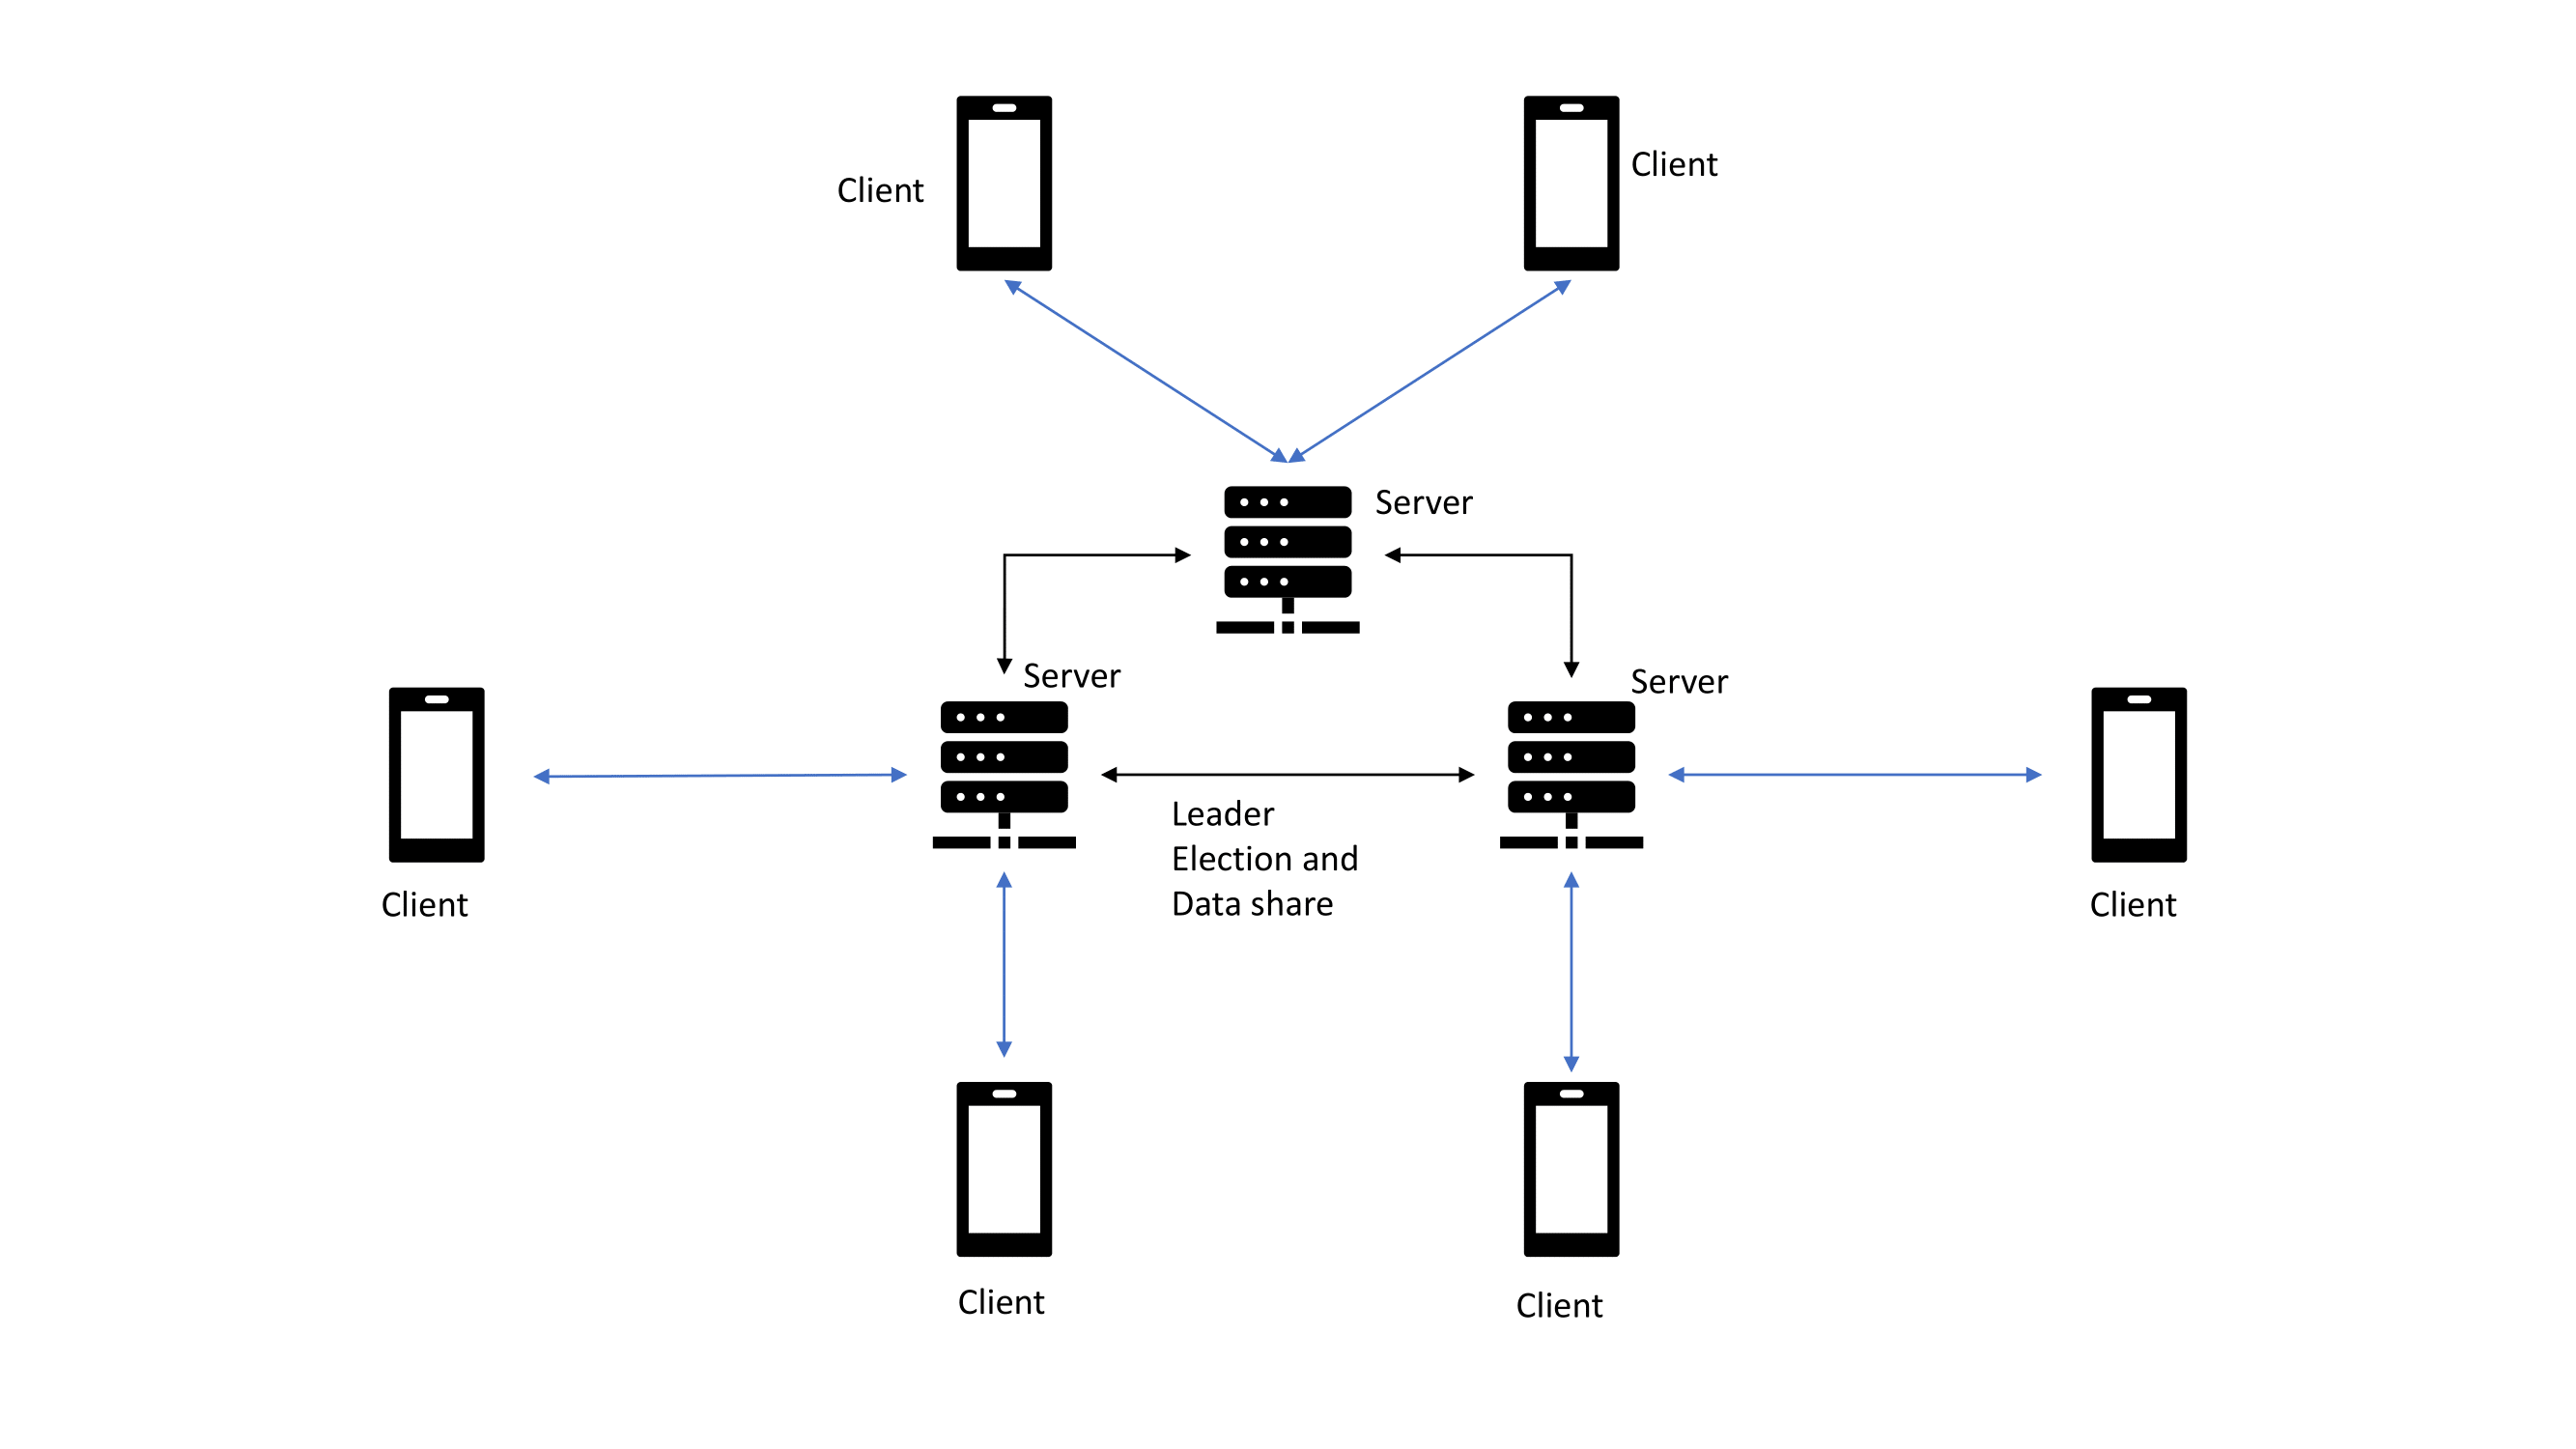
\includegraphics[width=\textwidth]{images/Architecture.png}
\caption{Architecture showing the system interaction.} \label{fig1}
\end{figure}



%
% ---- Bibliography ----
%
% BibTeX users should specify bibliography style 'splncs04'.
% References will then be sorted and formatted in the correct style.
%
% \bibliographystyle{splncs04}
% \bibliography{mybibliography}
%
%\begin{thebibliography}{8}
%\end{thebibliography}
\end{document}
